\documentclass[FM,MP]{tulthesis}  % Magisterský projekt fakulty mechatroniky
\usepackage[czech]{babel}  % Česká šablona dokumentu
\usepackage[utf8]{inputenc}  % Česká diakritika
\usepackage{graphicx}  % Tvorbě tabulek
\usepackage{float}  % Ukotvení věcí na svém místě (obrázky, tabulky, grafy, ...)
\usepackage{hyperref}  % Klikací odkazy v obsahu a referencích
\usepackage{gensymb}  % Pro stupne celsia
\usepackage{url}  % Pro lomeni adres url

\TULtitle{Zabezpečovací systém pomocí mobilního telefonu}{Security system using a mobile phone}
\TULprogramme{N2610}{Elektrotechnika a informatika}{Electrical Engineering and Informatics}
\TULbranch{1802T007}{Informační technologie}{Information Technology}
\TULauthor{Bc. Tomáš Moravec}
\TULsupervisor{doc. Ing. Josef Chaloupka, Ph.D.}
\TULyear{2017}

\begin{document}
\ThesisStart{male}

\begin{acknowledgement}
Děkuji vedoucí práce panu doc. Ing. Josefu Chaloupkovy, Ph.D. za odborné vedení a poskytnuté informace při zpracování magisterského projektu.
\end{acknowledgement}

% Abstrakt

\begin{abstractCZ}
Práce se zabývá problematikou zabezpečovacího systému, postaveného na platformě Arduino, řízeného z desktopové aplikace a s možností monitorování pomocí mobilní aplikace. Komunikace mezi zabezpečovacím systémem a mobilní aplikací má být realizována pomocí mobilního telefonu. V úvodu jsou definovány základní pojmy a požadované vlastnosti, na jejichž základě byly objednány jednotlivé komponenty. První část práce je věnována snaze o využití mobilního telefonu, jako prostředníka pro připojení do mobilní datové sítě. Tato cesta se ukázala jako slepá a byla tedy zvolena druhá alternativa, komunikace pomocí samostatného GPRS modulu. Výstupem práce je firmware, který řídí zabezpečovací systém a zajišťuje komunikaci, a desktopová aplikace pro úplné řízení zabezpečovacího systému. Poslední část, tedy mobilní aplikace zůstává nedokončená.

\end{abstractCZ}

\vspace{2cm}

\begin{abstractEN}

\end{abstractEN}

\tableofcontents
\clearpage

\begin{abbrList}
\textbf{SMS} & Short message service, služba krátkých textových zpráv\\
\textbf{GSM} & Groupe Spécial Mobile, globální systém pro mobilní komunikaci\\
\textbf{GPRS} & General Packet Radio Service, služba pro přenos dat v mobilní síti\\
\textbf{IDE} & Integrated development environment, integrované vývojové prostředí\\
\textbf{LED} & Light-Emitting Diode, dioda emitující světlo\\
\textbf{PIR} & Passive infrared sensor, infračervený sensor pohybu\\
\textbf{LAN} & Local Area Network, místní počítačová síť\\
\textbf{GBS} & Glass break detector, detektor rozbití skla\\
\end{abbrList}

% Úvod

\chapter{Úvod}
Téma bylo vypsáno doc. Ing. Josefem Chaloupkou, Ph.D. a zaujalo mne díky své tématické návaznosti na mou bakalářskou práci s názvem \uv{Koncept nízkonákladového sledovacího zařízení pro osobní automobily} \cite{Bachelor thesis}. V bakalářské práci jsem se věnoval vývoji sledovacího zařízení na založeného na platformě Arduino, které bylo komunikovalo pomocí SMS zpráv s mobilním telefonem. Dalším logickým krokem pro mne bylo, jak uvádím v závěru své bakalářské práce, řízení z desktopové aplikace, případně z mobilní aplikace, skrze mobilní datovou síť. Po konzultaci s vedoucím jsem byl obeznámen s tím, že tato práce mi nejen umožní navázat na předešlou práci bakalářskou, ale i prozkoumat možnosti využití starých, levných a nepoužívaných mobilních telefonů, jako náhradu za mnohdy drahé GPRS moduly. Nadchla mě myšlenka, že by bylo možné vzít starý nepoužívaný telefon, který má mnoho lidí ve vlastnictví, z důvodu neustálého obměňování za nejnovější modely, a nalézt pro něj smysluplné využití. Proto jsem se ihned přihlásil o toto zadání.

% Zabezpečovací systém
\chapter{Zabezpečovací systém}
Zabezpečovací systém, někdy také elektronická zabezpečovací signalizace, je zařízení, které vizuálně nebo akusticky vyhlašuje poplach a dává na vědomí, že nastaly nějaké potíže nebo došlo ke splnění sledované podmínky \cite{Security alarm}. Jde tedy o zařízení, které slouží k ochraně osob a majetku. Systém je řízen ústřednou a může se spustit analogovou (např. dveřní čidlo) i digitální (detektor pohybu) detekcí. Komunikace mezi detektory a ústřednou může být vedena kabelem, bezdrátově anebo kombinací předešlých způsobů, tj. jeden detektor může být připojen kabelem a druhý bezdrátově \cite{Electronic security system}.

\section{Ústředna}
Ústředna je „mozek“ celého systému, který je propojen s ostatními prvky systému kabely nebo bezdrátově. Obstarává komunikaci mezi jednotlivými komponenty systému, má v integrované paměti uložené nejdůležitější nastavení \cite{Electronic security system}. V závislosti na připojených komponentech pak může různě reagovat na splnění sledovaných podmínek. Často býva vybavena jenom tím nejnutnějším pro vyvolání poplachu, to ať už akustyckého (siréna), nebo tichého (informování majitele) \cite{Security alarm}.

\section{Ovladač}
Ovladač je prvek, který slouží k ovládání a případně též k programování ústředny. Dnešní alarmy je možné ovládat několika způsoby. Jako ovladač se nejčastěji používá klávesnice vybavená tlačítky, případně čtečkou (čipovými kartami a přívěšky) nebo též dálkové ovládání. U některých systémů se dá přes klávesnici provést nastavení celého systému. Klávesnice slouží k zastřežení i odstřežení systému \cite{Electronic security signalisation}. Dalšími způsoby je ovládání přes internet, kdy se většinou používá integrované webové rozhraní, ke kterému se uživatel může připojit po zadání hesla, nebo ovládání přes mobil (SMS příkazy) \cite{Bachelor thesis}.

\section{Detektor}
Detektor je prvkek systému, který je rozmístěn v hlídaném objektu a má za úkol reagovat aktivací při narušení (otevření, pohyb, rozbití atd.) a to tak, že tuto informaci předají ústředně, která ji následně zpracuje \cite{Electronic security signalisation}. Nejčastěji používané detektorové prvky jsou:

\begin{itemize}
\item Magnetický kontakt (dveřní čidlo)
\item Detektor pohybu (PIR detektor)
\item Detektor tříštění skla (GBS detektor)
\item Detektor plynu
\item Infra závora
\end{itemize} 

\section{Komunikátor}
Komunikátor je zařízení, které předává mimo objekt informaci o narušení objektu, případně o odchylce od normálního provozního stavu zabezpečovacího systému \cite{Electronic security signalisation}. Nejčastější typy komunikátorů jsou:

\begin{itemize}
\item GSM komunikátor
\item LAN komunikátor
\item Telefonní komunikátor
\item Komunikátor využívající radiové sítě s vyhrazenou frekvencí
\end{itemize} 

% Požadované vlastnosti a zvolené komponenty

\chapter{Požadované vlastnosti a zvolené komponenty}
V následující části se zaměřím na požadované vlastnosti zabezpečovacího zařízení a jaké komponenty byly na jejich základě zvoleny.

\section{Hardware}
Z úvodní části je jasné, že kompletní zabezpečovací systém musí obsahovat detektory, komunikátor a ústřednu. Rozebereme si tedy jednotlivé části.

\subsection{Ústředna}
Požadavky na ústřednu jsou takové, že musí být schopná komunikovat jak s desktopovou aplikací, tak s mobilní aplikací a zároveň musí řídit a zpracovávat jednotlivé komponenty. Zadání informuje o použití vývojové platformy Arduino, která je se svými periferiemi a čipem Atmega, více než vhodnou pro tyto účely. Firmware pro ústřednu bude psán v jazyku  C a C++ s nadstavbou Wiring (knihovny pro řízení hardwaru) \cite{Wiring}, vývojové prostředí Visual Studio 2017 s rozšířením Visual Micro \cite{Visual Micro}. Arduino Uno bylo zakoupeno v obchodu \url{arduino-shop.cz}.

\paragraph{Zvolená ústředna:}
\begin{itemize}
\item Arduino Uno Rev3 (700 Kč s DPH)
\end{itemize} 

\subsection{Detektory}
Požadavky nejsou kladeny pouze na samotné detektory, ale také na spínače, kterými bude možné spínat různá zařízení. Jako spínací prvky není nutné volit jednotlivé komponenty, stačí připravit implementaci jejich spínání. V případě detektorů musí být možné připojit libovolý detektor, který lze nastavit jako spínací (normálně rozepnutý), nebo rozpínací (normálně sepnutý). Pro testovací účely byly zvoleny dva detektory, každý jednoho typu. Sensor PIR byl objednán z číny.

\paragraph{Zvolené detektory:}
\begin{itemize}
\item Dveřní čidlo (rozpínací), (poskytl vedoucí)
\item PIR detektor (spínací), (25 Kč s DPH)
\end{itemize} 

\subsection{Komunikátor}
Požadavek na komunikátor je přenos dat do počítače a přes mobilní data. Zadání jako hlavní komunikátor určuje mobilní telefon, pomocí kterého máme umožnit ústředně datové přenosy. Zvolen byl nový a zároveň nejlevnější mobilní telefon na trhu, kteý byl zakoupen z obchodu Alza.cz. Pro případ neúspěchu, při získávání zdrojů mobilního telefonu, byla zvolena alternativa v podobě GSM/GPRS modulu, který byl zakoupen z Číny, dodací doba této součástky, stejně jako na všechny ostatní, byla přes jeden kalendářní měsíc.

\paragraph{Zvolené komunikátory:}
\begin{itemize}
\item Mobilní telefon STK R45i Black (449 Kč s DPH)
\item GSM/GPRS modul (290 Kč s DPH)
\end{itemize} 

\section{Software (Ovladač)}
Výše zmíněné prvky musí  být řízeny ovladačem, v mém případě aplikací jak desktopovou tak mobilní. Proto bude následující část rozdělena do těchto dvou částí.

\subsection{Desktopová aplikace}
Na desktopovou aplikaci jsou kladeny požadavky tak, aby byla schopna využít všech možností, které nám ústředna poskytuje. Musí být schopna kompletní správy a nastavení jednotlivých komponent (spínače a senzory) a tím pádem i komunikaci s ní. Cílový operační systém jsem si zvolil Windows 10, jakožto ve škole nejrozšířenější, programovací jazyk C\# a vývojové prostředí Visual Studio 2017. Jednotlivé požadavky kladené na desktopovou aplikaci lze nalézt níže.

\paragraph{Požadavky na desktopovou aplikaci:}
\begin{itemize}
\item Sledování aktuálních stavů komponent
\item Přidávání nových komponent
\item Odstraňování stávajících komponent
\item Přejmenování komponent
\item Změna pinů komponent
\item Změna nastavení senzorů jako spínacích či rozpínacích
\item Notifikace v případě změny stavů senzorů
\item Přepínání stavů spínačů
\item Připojování a odpojování ke zvolené ústředně
\end{itemize} 

\subsection{Mobilní aplikace}
Mobilní aplikace je učena pouze jako monitorovací zařízení, ze kterého bude možné sledovat stavy jednotlivých senzorů, případně spínač spínače. Její návrh je tedy značně jednodušší oproti komplexnější desktopové aplikaci. Cílový operační systém jsem zvolil Android, jakožto nerozšířenější, programovací jazyk Java a vývojové prostředí a Android Studio.

\paragraph{Požadavky na mobilní aplikaci:}
\begin{itemize}
\item Sledování aktuálních stavů komponent
\item Přepínání stavů spínačů
\item Připojování a odpojování ke zvolené ústředně
\end{itemize} 

% Hardware a firmware

\chapter{Hardware a firmware}

\section{Využití mobilního telefonu}

\subsection{První rozbor}

\subsection{Kontaktování výrobce}

\subsection{Hlubší rozbor}

\subsection{Závěr rozboru}

\section{Zapojení}

\subsection{Blokové schéma}

\subsection{Výsledný prototyp}

\section{Firmware}

\subsection{Komunikace}

\subsection{Notifikace}

% Desktopová aplikace

\chapter{Desktopová aplikace}

% Mobilní aplikace

\chapter{Mobilní aplikace}

%Softwarový návrh



\chapter{Softwarový návrh}
V programové části se nejdříve zaměřím na popis programovacího jazyka, vývojové prostředí, ve kterém bude software tvořen a dále na postupy při tvorbě jednotlivých částí, problémy se kterými jsem se u nich setkal a jakým způsobem jsem je vyřešil.

\section{Programovací jazyk}
Vývoj softwaru bude probíhat v programovacím jazyce C s nadstavbou vývojové platformy Wiring  (knihovna Wire)\cite{Arduino acce}, která jazyk rozšiřuje o nové příkazy, pro přímé řízení hardwarových součástek, vše zastřešeno sadou knihoven \cite{Arduino lib} (od tvůrců desky Arduino), které přidávají nové funkce, aby potencionální vývojář nepotřeboval hlubší znalosti programování a hardwaru. Tento kompletní balík příkazů \cite{Arduino lang} je někdy také nazýván programovacím jazykem Arduino \cite{Arduino intro}.

\section{Vývojové prostředí Arduino}
Pro vývoj softwaru budu používat oficiální vývojové prostředí, od tvůrců desky Arduino s identickým názvem Arduino \cite{Arduino soft}. Jedná se o počítačový software s otevřeným zdrojovým kódem (open-source) \cite{Arduino source}, určený k jednoduchému psaní a nahrávání zdrojových kódů na desku. Prostředí lze nainstalovat na operační systém Windows, MAC a Linux. Z vlastní zkušenosti vyjmenuji výhody, mezi které patří zvýraznění a barevné rozlišení jednotlivých příkazů, plná podpora vývojové platformy Wiring, podpora všech oficiálních i neoficiálních desek Arduino, zabudovaný klient pro komunikaci na sériové lince a dalších funkce. Nevýhodou je absence předvídání a dokončování kódu (predikce), nápověda při volání částí programu (funkcí, knihoven atd.), nemožnost krokování programu a velice obecné chybové hlášky, kvůli kterým je náročné odhalit případné chyby.

\begin{figure}[H]
\begin{center}
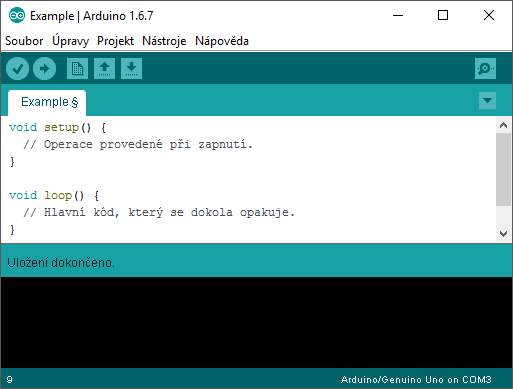
\includegraphics[width=0.8\textwidth]{images/arduino-ide.png}
\caption{Ukázka z vývojového prostředí Arduino}
\label{image}
\end{center}
\end{figure}

% Hlavní program

\section{Hlavička programu}
V hlavičce jsou definovány všechny globální proměnné, které jsou určeny primárně ke změnám pomocí příkazů SMS. Především se ale v této části nachází textové řetězce, které jsou na jednom uceleném místě, určené například k jednoduchému rozšíření do jiného jazyka, nebo k úpravám již stávajících testových řetězců.

\section{Hlavní funkce programu}
Pod hlavičkou programu se nachází zdrojové kódy, které tvoří jádro celého programu, hlavními částmi jsou inicializace (setup), která slouží pro uvedení do výchozího stavu a smyčka (loop), která dle situace volá ostatní podprogramy (funkce). Níže detailně popíši všechny funkce hlavního programu, jaký je jejich účel, jaké mají vstupní parametry a co je jejich výstupem.

\subsection{Inicializace (setup)}
Inicializace slouží k uvedení zařízení do výchozího stavu a načtení nastavení a dat z paměti. Jako první se nastaví všechny piny, které se budou používat jako výstupní, dále se všechny piny, používané pro signalizace diodamy LED, nastaví do logické nuly. Je zahájen komunikační rámec seriové linky, pro komunikaci s modulem GPS/GSM/GPRS, popřípadě s počítačem, který slouží pro monitorování stavu.  Následuje přepnutí řídících pinů do logické jedna, které znamenají, aby se modul připojil do sítě. Nakonec je zařízení přepnuto do režimu GSM, zavoláním funkce changeMode, s textovým parametrem GSM. Funkce pracuje pouze s globálními proměnnými a nevrací žádný výstup.

\subsection{Hlavní smyčka (loop)}
Hlavní smyčka je jádrem, které spojuje všechny funkce do jednoho celku, zastřešuje jejich funkčnost a zajištuje vzájemnou provázanost. Kód je rozdělen na části podle režimu modulu, pokud je v režimu GSM, čeká na příchozí komunikaci. Pokud jí obdrží, načte kompletně jeden komunikační rámec a poté ověří, zda se jedná o SMS, pokud ano, jsou volány postupně další funkce, které načtou hlavičku, obsah a nakonec požadavek v obsahu těla SMS vykonají. Druhá část je částí GPS, kdy se čeká pouze na plně načtená data z přerušení. Pokud jsou data kompletní, začne zpracování a výpočet validních dat GPS, pokud jich je dostatek a je ověřena jejich validita, je modul přepnut do režimu GSM a předá mu informace o poloze. Funkce pracuje pouze s globálními proměnnými a nevrací žádný výstup.


\paragraph{Vstupní parametr funkce:}
\begin{itemize}
\item textový řetězec String s kompletním příkazem pro modul.
\end{itemize}

% Režim GSM

\section{Funkce v režimu GSM}
Níže detailně popíši všechny funkce režimu GSM, jaký je jejich účel, jaké mají vstupní parametry a jaká je jejich návratová hodnota.

\subsection{Rozpoznání nové SMS (recognizeSmsNew)}
Funkce obstarává zjištění, zda v režimu GSM dorazila nová SMS, to dává modul navědomí textovým řetězcem +CMTI, viz softwarová dokumentace \cite{SIMCOM SW}. Po registrování nové SMS je modulu zaslána žádost AT+CMG=1 \cite{SIMCOM SW}, která slouží k vyžádání hlavičky a těla textové zprávy. Funkce pracuje s globálními proměnnými a nevrací žádný výstup.

\subsection{Rozpoznání hlavičky SMS (recognizeSmsHeader)}
Pokud byla obdržena nová SMS, očekává se přijetí, její hlavičky. Pokud tak nastane, je z hlavičky vyčteno telefonní číslo odesílatele, na které bude později odeslána odpověď SMS. Číslo je uloženo do globální proměnné a je nastaven příznak čtení SMS, tedy značí, že je program připraven číst obsah. Funkce pracuje pouze s globálními proměnnými a nevrací žádný výstup.

\subsection{Rozpoznání obsahu SMS (recognizeSmsContent)}
Po rozpoznání hlavičky SMS a nastavení příznaku čtení, je očekáván obsah zprávy. Modul posílá zprávu ihned po hlavičce, ale v případě, že by se tak nestalo, proběhne ověření, zda se opravdu jedná o zprávu SMS zkontrolováním obsahu zprávy, zda není prázdný (znak nového řádku vždy chodí před příkazem) a zda je nastaven příznak čtení. Poté jsou příchozí data vyčtena a označena za tělo zprávy SMS. Funkce pracuje pouze s globálními proměnnými a nevrací žádný výstup.

\subsection{Vykonání obsahu SMS (executeSmsContent)}
V případě, že je zpráva kompletní, je zavolána funkce pro vykonání obsahu SMS. Zde je textový řetězec ve zprávě SMS, dle jazyka, porovnáván s textovými řetězci v globálních proměnných, kde se ověřují pouze znaky, nezáleží tedy zda jsou písmenka malá, nebo velká. Pokud obsah sedí do jednoho z definovaných textů, je vykonán požadavek. Například pokud bude přijata zpráva \uv{Kde jsi?}, bude obratem odeslána odpověď: \uv{Probíhá lokalizace, poloha bude zaslána během několika minut}, odesláním textu do funkce sendSMS(), následně je modul přepnut do režimu GPS a tím ukončena činnost této části kódu. Funkce pracuje pouze s globálními proměnnými a nevrací žádný výstup.

\subsection{Odeslání SMS (sendSMS)}
Funkce přepne modul do textového režimu, bude tedy očekávat odeslání textového řetězce, dále odešleme informaci pro odeslání SMS na telefonní číslo, uvedeném v příkazu. Čekáme na odpověď, když dorazí, je modul v režimu přijímání textu a jeho ukončení je možné pouze kombinací kláves CTRL+C, tato klávesová zkratka má naštěstí svou hodnotu v tabulce ASCII, tedy hodnotu 42. Funkce odešle všechen text, který obdržela na vstupu v textovém řetězci, poté je odeslán ukončovací příznak CTRL+C. Tím je SMS zpráva úspěšně odeslána do modulu, který již dále převezme režii, separovaně od úloh řídící jednotky. Mezi každým krokem jsou nastaveny časové intervaly, definované v hlavičce, které slouží jako doba, kterou má modul na odpověď našeho požadavku. Funkce nevrací žádný výstup.

% Závěr

\chapter{Závěr}
V rešeršní části jsem definoval sledovací zařízení, seznámil jsem se s jeho historií i současností a definoval jsem vlastní požadované vlastnosti, které pro mě hrají důležitou roli při tvorbě zmíněného zařízení. Nakonec jsem se seznámil s platnými standardy a technickými předpisy související s tématem práce. Průzkumem trhu jsem vytvořil kategorie sledovacích zařízení, dle jejich cenových hladin a vlastností těmto hladinám vlastním. Definoval jsem ideální nízkonákladové zařízení, kdy jsem každé požadované vlastnosti přiřadil maximální počet bodů a poté jsem vyhodnotil nejkvalitnější, mnou vybrané konkurenční výrobky, kterým jsem udělil příslušný počet bodů v každé kategorii, kdy zařízení s nejvyšší cenou získalo nejvyšší počet bodů (72/100) a zařízení s cenou nejnižší, získalo bodů nejméně (50/100).

Na základě častých konzultací s vedoucí práce, jsem navrhl koncept cílového zařízení, doporučil realizační postupy, vybral hardware, nebo uvedl více možností jeho výběru, kterými může být dosaženo výsledného zařízení. Následně jsem zvolil komunikační prostředky a architekturu jednotlivých komponentů. Nakonec jsem pro koncept vybral vhodné osazení ve voze a vytvořil blokové zapojení komponentů. Vše jsem pečlivě vybíral tak, aby byla výrobní cena co nejnižší, nejlépe aby se držela pod hranicí 1 000 Kč, ale vlastnosti dosahovaly ideálního sledovacího zařízení.

Na základě konceptu jsem zvolil nejvhodnější komponenty pro vývoj prototypu, které jsem následně zakoupil. Nastudoval jsem použitý programovací jazyk, včetně knihoven, které jsem později použil ve svém kódu. Před psaním kódu jsem popsal programové prostředí, ve kterém bude vývoj probíhat, po dopsání vlastního kódu jsem podrobně popsal všechny funkce programu, jejich možnosti, vlastnosti, vstupní parametry a návratové hodnoty. 

Funkční prototyp jsem otestoval v běžném provozu, kdy 14 dní nepřetržitě běželo bez jediného pádu či problému a poté jsem testování ukončil. Dále jsem změřil spotřebu jednotlivých komponentů i celého zařízení a naměřil teoretickou výdrž až 200 dní nepřetržitého provozu, při použití s nejslabší používanou autobaterii o kapacitě 50 Ah, která po celou dobu nebude dobíjena.

Nakonec jsem své zařízení ohodnotil stejnou metodikou, kterou jsem použil pro hodnocení konkurenčních výrobků, přičemž mé sledovací zařízení získalo 92 bodů.

Vývoj sledovacího zařízení má před sebou ještě dlouhou cestu do finální podoby, ale věřím, že v práci budu pokračovat a vše dokončím dle mých původních představ.

% Literatura

\addcontentsline{toc}{chapter}{Literatura}
\begin{thebibliography}{10}
\bibitem{Bachelor thesis}MORAVEC, Tomáš. Koncept nízkonákladového sledovacího zařízení pro osobní automobily: The concept of a low cost tracking device for personal cars. Liberec: Technická univerzita v Liberci, 2016.
\bibitem{Security alarm}Security alarm. Wikipedia [online]. [cit. 2017-05-23]. Dostupné z: \url{https://en.wikipedia.org/wiki/Security_alarm}
\bibitem{Electronic security system}Elektronické zabezpečovací systémy [online]. , 1 [cit. 2017-05-23]. Dostupné z: \url{http://www.ezasys.cz/elektronicke-zabezpecovaci-systemy/}
\bibitem{Electronic security signalisation}Elektronická zabezpečovací signalizace. Wikipedia [online]. [cit. 2017-05-23]. Dostupné z: \url{https://cs.wikipedia.org/wiki/Elektronick\%C3\%A1\_zabezpe\%C4\%8Dovac\%C3\%AD_signalizace}
\bibitem{Wiring}Wiring [online]. [cit. 2016-05-08]. Dostupné z: \url{http://wiring.org.co/}
\bibitem{Visual Micro}Visual Micro [online]. [cit. 2017-05-23]. Dostupné z: \url{http://www.visualmicro.com/}



\bibitem{guide}A Guide To The Global Positioning System. Radioshack [online]. [cit. 2016-05-09]. Dostupné z: \url{http://support.radioshack.com/support\_tutorials/gps/gps\_tmline.htm}
\bibitem{Arduino intro}Arduino introduction. Arduino [online]. [cit. 2016-05-08]. Dostupné z: \url{https://www.arduino.cc/en/Guide/Introduction}
\bibitem{Arduino lib}Arduino libraries. Arduino [online]. [cit. 2016-05-08]. Dostupné z: \url{https://www.arduino.cc/en/Reference/Libraries}
\bibitem{Arduino lang}Arduino programming language. Arduino [online]. [cit. 2016-05-08]. Dostupné z: \url{https://www.arduino.cc/en/Reference/HomePage}
\bibitem{Arduino schematic}ARDUINO LLC. Arduino Schematic [online]. 1 s. [cit. 2016-05-07]. Dostupné z: \url{https://www.arduino.cc/en/uploads/Main/Arduino\_Uno\_Rev3-schematic.pdf}
\bibitem{Arduino soft} Arduino software. Arduino [online]. [cit. 2016-05-08]. Dostupné z: \url{https://www.arduino.cc/en/Main/Software}
\bibitem{Arduino source}Arduino source code. GitHub [online]. [cit. 2016-05-08]. Dostupné z: \url{https://github.com/arduino/Arduino/tree/1.6.8}
\bibitem{Atmega datasheet}ATMEL CORPORATION. ATmega48A/PA/88A/PA/168A/PA/328/P Datasheet [online]. 2015, 660 s. [cit. 2016-05-07]. Dostupné z: http://www.atmel.com/images/Atmel-8271-8-bit-AVR-Microcontroller-ATmega48A-48PA-88A-88PA-168A-168PA-328-328P\_ datasheet\_Complete.pdf
\bibitem{geographic}Geographic coordinate system. Wikipedia [online]. [cit. 2016-05-09]. Dostupné z: \url{https://en.wikipedia.org/wiki/Geographic\_coordinate\_system}
\bibitem{gpsCommon}Global Positioning System. Wikipedia [online]. [cit. 2016-05-09]. Dostupné z: \url{https://en.wikipedia.org/wiki/Global\_Positioning\_System}
\bibitem{ROBOT SW}GPS/GPRS/GSM Module V3.0 (SKU:TEL0051). DFRobot Wiki [online]. [cit. 2016-05-07]. Dostupné z: \url{http://www.dfrobot.com/wiki/index.php/GPS/GPRS/GSM\_Module \_V3.0\_(SKU:TEL0051)}
\bibitem{ROBOT schematic}DFROBOT. GSM+GPRS+GPS V3.0 schematic [online]. Shanghai, 2013, 1 s. [cit. 2016-05-07]. Dostupné z: \url{http://www.dfrobot.com/image/data/TEL0051/GSM+GPRS+GPS\%20SIM908\%20V3.0.pdf}
\bibitem{I2cdevlib}STOFFREGEN, Paul. I2cdevlib - MPU6050 [online]. 2012, 2016-04-07 [cit. 2016-05-08]. Dostupné z: \url{https://github.com/jrowberg/i2cdevlib/tree/master/Arduino/MPU60-50}
\bibitem{LaTeX}SATRAPA, Pavel. LaTeX pro pragmatiky [online]. 2011, 87 s. [cit. 2016-05-07]. Dostupné z: \url{http://www.nti.tul.cz/~satrapa/docs/latex/latex-pro-pragmatiky.pdf}
\bibitem{Arduino acce}ARDUINO LLC. MPU-6050 Accelerometer + Gyro [online]. [cit. 2016-05-08]. Dostupné z: \url{http://playground.arduino.cc/Main/MPU-6050}
\bibitem{glonass}DALY, P. Navstar GPS and GLONASS [online]. 1993 [cit. 2016-05-09]. Dostupné z: \url{http://ieeexplore.ieee.org/stamp/stamp.jsp?arnumber=285510}
\bibitem{CSR}CSR PLC. NMEA Reference Guide [online]. 2. Cambridge: CSR plc, 2011, 50 s. [cit. 2016-05-07]. Dostupné z: \url{http://www.inventeksys.com/wp-content/uploads/2012/05/NMEA-Reference-Manual-CS-129435-MA-2.pdf}
\bibitem{SIFT}SIRF TECHNOLOGY, INC. NMEA Reference Manual [online]. 2.1. San Jose., 2007, 27 s. [cit. 2016-05-07]. Dostupné z: \url{https://www.sparkfun.com/datasheets/GPS/NMEA\%20Reference\%20Manual-Rev2.1-Dec07.pdf}
\bibitem{correct}BYRNE, Jonathan. Position error with GPS/GSM v3. In: Dfrobot [online]. [cit. 2016-05-09]. Dostupné z: \url{http://www.dfrobot.com/forum/viewtopic.php?f=2\&t=1528\&p=7729\#p7693}
\bibitem{Pruvodce arduinem}VODA, Zbyšek. Průvodce světem Arduina [online]. Vydání první. Bučovice: Martin Stříž, 2015 [cit. 2016-05-07]. ISBN 978-80-87106-90-7.
\bibitem{SIMCOM SW}SIMCOM WIRELESS SOLUTIONS. SIM908 AT Command Manual [online]. Jinzhong, 2011, 249 s. [cit. 2016-05-07]. Dostupné z: \url{http://www.dfrobot.com/image/data/TEL0051/3.0/SIM908\_AT\%20Command\%20Manua\_V1.01.pdf}
\bibitem{SIMCOM HW}SIMCOM WIRELESS SOLUTIONS. SIM908 Hardware Design [online]. 2. Jinzhong, 2012, 53 s. [cit. 2016-05-07]. Dostupné z: \url{http://www.niplesoft.net/blog/wp-content/uploads/2016/02/SIM908-Hardware-Design-V2.00-1.pdf}
\bibitem{SoftReset}Software Reset Library for Arduino. GitHub [online]. [cit. 2016-05-08]. Dostupné z: \url{https://github.com/WickedDevice/SoftReset}
\bibitem{LaTeX}SATRAPA, Pavel. Stručný přehled příkazů LaTeXu [online]. 2011, 2 s. [cit. 2016-05-07]. Dostupné z: \url{http://www.nti.tul.cz/~satrapa/docs/latex/latex-prehled.pdf}
\bibitem{gps}The global positioning system: a shared national asset : recommendations for technical improvements and enhancements. Washington, D.C.: National Academy Press, 1995. ISBN ISBN 0-309-05283-1.
\bibitem{what}What is a GPS? How does it work? Library of congress [online]. [cit. 2016-05-09]. Dostupné z: \url{http://www.loc.gov/rr/scitech/mysteries/global.html}
\end{thebibliography}

% Příloha

\appendix
\chapter{Obsah přiloženého CD}
Struktura a obsah adresářů je následující:

\paragraph{/Dokumentace}\mbox{}\\\mbox{}\\
Text bakalářské práce ve formátu pdf.

\paragraph{/Software}\mbox{}\\\mbox{}\\
Zdrojové kódy rozděleny do více kategorií.

\paragraph{/Software/Dokumentace (Datasheets)}\mbox{}\\\mbox{}\\
Softwarová a hardwarová dokumentace použitých součástek.

\paragraph{/Software/Komunikační software (Hyper-Terminal)}\mbox{}\\\mbox{}\\
Komunikační software, sloužící pro ladění sledovacího zařízení z počítače.

\paragraph{/Software/Nepoužité zdrojové kódy (Testovací)}\mbox{}\\\mbox{}\\
Zdrojové kódy, sloužily jako testovací, nebo zatím nejsou potřeba (akcelerometr).

\paragraph{/Software/Software}\mbox{}\\\mbox{}\\
Hlavní software, nahraný ve sledovacím zařízení.

\end{document}